\documentclass[letterpaper]{article}

\usepackage{aaai}
\usepackage{amsmath}
\usepackage{amssymb}
\usepackage{amsthm}
\usepackage{courier}
\usepackage{graphicx}
\usepackage{helvet}
\usepackage{times}
\usepackage{verbatim}

\newtheorem{definition}{Definition}
\newtheorem{example}{Example}
\newtheorem{formula}{Formula}
\newtheorem{problem}{Problem}

%\setlength\parindent{0pt}
\frenchspacing

\setlength{\pdfpagewidth}{8.5in}
\setlength{\pdfpageheight}{11in}

\pdfinfo{
/Title Rough Set Semantics for Identity Management on the Web
/Author Wouter Beek, Stefan Schlobach, Frank van Harmelen}
\setcounter{secnumdepth}{0}

\begin{document}

\title{Rough Set Semantics for Identity Management on the Web}
\author{Wouter Beek \and Stefan Schlobach \and Frank van Harmelen\\
Vrije Universiteit Amsterdam\\
De Boelelaan 1081a\\
1081HV Amsterdam\\
The Netherlands}
\maketitle
\begin{abstract}
\begin{quote}
Identity relations are at the foundation of the Linked Open Data initiative and on the Semantic Web in general. They allow the interlinking of alternative descriptions of the same thing. However, many practical uses of \verb|owl:sameAs| are known to violate its formal semantics. We propose a method that assigns meaning to (the subrelations of) an identity relation using the predicates of the dataset schema. Applications of this approach include automated suggestions for asserting/retracting and quality assessment. We also describe an experimental design for this approach.
\end{quote}
\end{abstract}

\section{Introduction}
\label{sec:introduction}

Identity relations are at the foundation of the Linked Open Data initiative and of the Semantic Web in general \cite{bizer_cyganiak_heath_2007}. They allow the interlinking of alternative descriptions of the same thing. However, the traditional notion of identity (expressed by \verb|owl:sameAs| \cite{motic_paterschneider_grau_2012}) is often problematic, e.g. when objects are considered the same in some contexts but not in others. The standing practice in such cases is to use weaker relations of relatedness (e.g. \verb|skos:related|). Unfortunately, this limits reasoners in drawing inferences.

According to the traditional semantics of the identity relation, identical terms can be replaced for one another in all non-modal contexts \emph{salva veritate}. Practical uses of \verb|owl:sameAs| are known to violate this strict semantics \cite{halpin_hayes_2010,halpin_hayes_mccusker_mcguinness_thompson_2010}.

\subsection{Previous work}
\label{sec:previous_work}

Existing research proposes the following solutions for the problem of identity relations in the Semantic Web. (1) Introduce weaker versions of \verb|owl:sameAs| \cite{halpin_hayes_2010,mccusker_mcguinness_2010} (e.g., \verb|skos:related|). (2) Restrict the applicability of identity relations to specific contexts. Identities are expected to hold within a named graph or within a namespace, but not necessarily outside of it \cite{halpin_hayes_2010,melo_2013}. (3) Introduce additional vocabulary that does not weaken but extend the existing identity relation \cite{halpin_hayes_2010}. For example, allow an explicit distinction to be made between mentioning a term and using a term (e.g. a car and a Web document describing that car). (4) Add domain-specific weaker versions of the identity relation \cite{mccusker_mcguinness_2010} (e.g., ``have the same medical use'' is weaker than ``are the same molecule''). (5) Adapt the modeling practice, possibly in a (semi-)automated way by adapting visualization and modeling toolkits to produce notifications upon reading data. This can for example be done by giving a warning upon importing an identity pair from an external resource. Alternatively, additional restrictions can be put on changing and creating data. For example adding an RDF link could require reciprocal confirmation from the maintainers of the respective datasets. \cite{halpin_hayes_2010,ding_shinavier_finin_mcguinness_2010}

Other related research focusses on the extraction of network properties of \verb|owl:sameAs| datasets \cite{ding_shinavier_shangguan_mcguinness_2010}, but these endeavors are not yet related to the semantics of the identity relation.

What these approaches have is common is that quite some work has to be done (adapting or creating standards, instructing modelers, converting existing dataset) in order to resolve some of the problems of identity. Our approach provides a way of dealing with the heterogeneous real-world usage of identity in the Semantic Web that is fully automated and that requires no changes to standards, modeling practices, or existing datasets.

\subsection{Research goals}
\label{sec:research_goals}

In developing our new approach we have the following research goals:

\begin{enumerate}
\item In an identity relation the pairs all look the same. We want to characterize subrelations of an identity relation in terms of the predicates that occur in the schema of the dataset.
\item Based on an existing identity relation we want to give semantically motivated suggestions for extending and/or retracting the identity relation.
\item We want to assess the quality of an identity relation based on the consistency in which it is applied to the data.
\end{enumerate}

\section{Approach}
\label{sec:approach}

In the following we shall consider an arbitrary graph $G$. The resources (excluding blank nodes) that occur as the subject term of some triple in $G$ are called $S_G$. We choose not to include blank nodes in our approach, since identity relations are almost never defined between them. The resources that occur as the predicate term of some triples in $G$ are called $P_G$. In the following we assume that $G$ is a fully materialized graph.

For illustrative purposes we shall use the IIMB dataset as it is used in the instance matching track of the Ontology Alignment Evaluation Initiative 2012 \cite{oaei_2012}. This dataset consists of eighty ontologies that are linked to a single base ontology. For each of these eighty links a reference mapping is available. The graphs $G$ are the result of merging the two linked graphs.

We will use the words `property' and `predicate' in order to denote slightly different things. A \emph{property} is taken to be a predicate-object pair. Examples of properties are ``is spoken in Germany'' and ``has a democratic form of government''. Examples of \emph{predicates} are ``is spoken in'' and ``form of government is''.

In theory it is possible to construct properties of arbitrary depth (in terms of the distance to the subject term) by using blank nodes to existentially quantify over intermittent resources. For example ``is spoken in a country with a democratic form of government'' is a property that quantifies over countries and that may be shared by the languages French and Dutch. In this paper we only consider properties of `depth one', i.e. properties that consists of a single predicate and object term.

\subsection{Shared properties and indiscernibility}
\label{sec:indiscernibility}

When we look at the triples that constitute a set of identity relations, we see that all links look the same. But when we take the triples in which the subject and object terms occur into account, we see that within the identity relation there may be different subrelations that we can identify in terms of the predicates that occur in the schema.

For instance, in the IIMB graphs there are some identical resources that share the property \verb|IIMBTBOX:spoken_in|, while other pairs share the property \verb|IIMBTBOX:form_of_government|. The set of pairs of resources that are spoken in the same language may even be disjoint from the set of pairs of resources that have the same form of government.

Note that we are not only interested in the properties that resources share with one other (e.g., where they are spoken, or which form of government they have), but we are also interested in resource pairs that share the same sharing properties. We can thus identify subsets of an identity relation based on differences in the sets of predicates relative to which they take resources to be \emph{indiscernible} from one another.

In the example above, one subset of the identity relation does not discern resources that are spoken in the same language, whereas another subset of the identity relation does not discern resources that have the same form of government.

As in rough set theory, we define indiscernibility as a set of pairs for which it is impossible to show the distinction. We therefore say that two resources are indiscernible with respect to a set of predicates $P$ ($IND(P)$, definition \ref{def:unary_indiscernibility}) in case they share the same properties. We say that two resource pairs are indiscernible ($IND(P^*)$, definition \ref{def:binary_indiscernibility}) in case both pairs are indiscernible for the same $P^* \subseteq \mathcal{P}(P_G)$.

\begin{definition}[Indiscernibility]
\begin{align}
IND(P) = \{
  \langle x, y \rangle \in S_G^2
\  \vert \ 
  \forall a \in P(a(x) = a(y))
\}
\label{def:unary_indiscernibility}
\\
IND(P^*) \  = \  \{
    \langle
      \langle x_1, y_1 \rangle,
      \langle x_2, y_2 \rangle
    \rangle \in (S_G^2)^2
  \  \vert \ 
\nonumber
\\
    \forall P \in P^*(P(x_1, y_1) = P(x_2, y_2))
  \}
\label{def:binary_indiscernibility}
\end{align}
\end{definition}

As explained above, for a given set of identity pairs there may be multiple pairs that have the same shared properties. These sets of predicates that are shared across resource pairs are considered to give a description of a specific subrelation of the identity relation. For example, in figure \ref{fig:indiscernibility_example} the subrelation $\{ \langle a, c \rangle, \langle b, c \rangle \}$ is characterized by $\mathcal{P}(\{ P \})$.

\begin{comment}
\begin{figure}[h!]
\centering
\label{fig:indiscernibility_example}
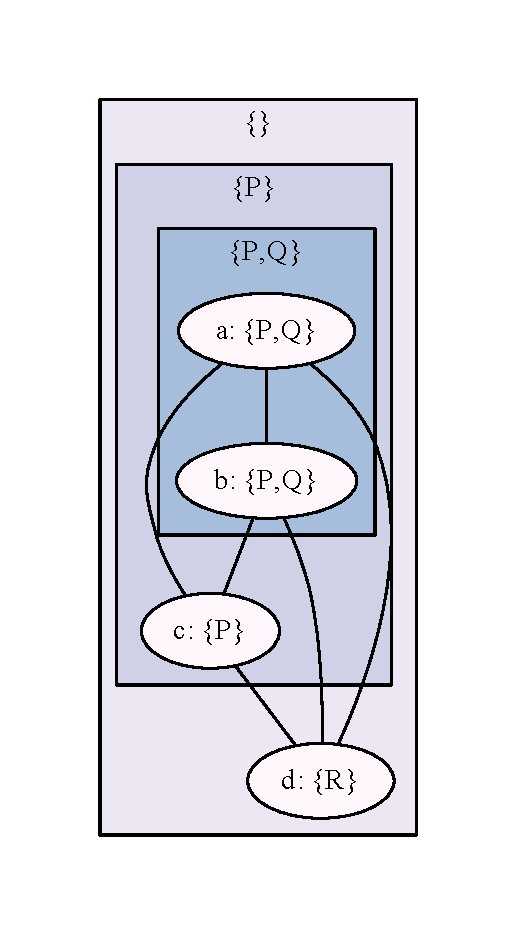
\includegraphics[scale=0.7]{indiscernibility_example}
\caption{This figure contains four resources, represented by nodes and annotated with the properties $P$, $Q$, and $R$ that apply to them. It also contains six pairs, represented as edges between the nodes (reflexive pairs are not shown). The edges are drawn inside squares that represent the indiscernibility sets to which they belong. For instance $\langle a, c \rangle$ and $\langle a, c \rangle$ belong to the same indiscernibility set $\{ P \}$, but $\langle a, b \rangle$ belongs to indiscernibility set $\{P, Q\}$.}
\end{figure}
\end{comment}

According to the standard definition, identical resources are indiscernible with respect to all properties. We take a given set of identity pairs and partition it into subsets which we can describe as being $P$-indiscernible, for $P \subseteq P_G$.

Figure \ref{fig:iimb_example} shows an example of a discernibility partitioning for a given identity relation.

\begin{figure*}
\label{fig:iimb_example}
\centering
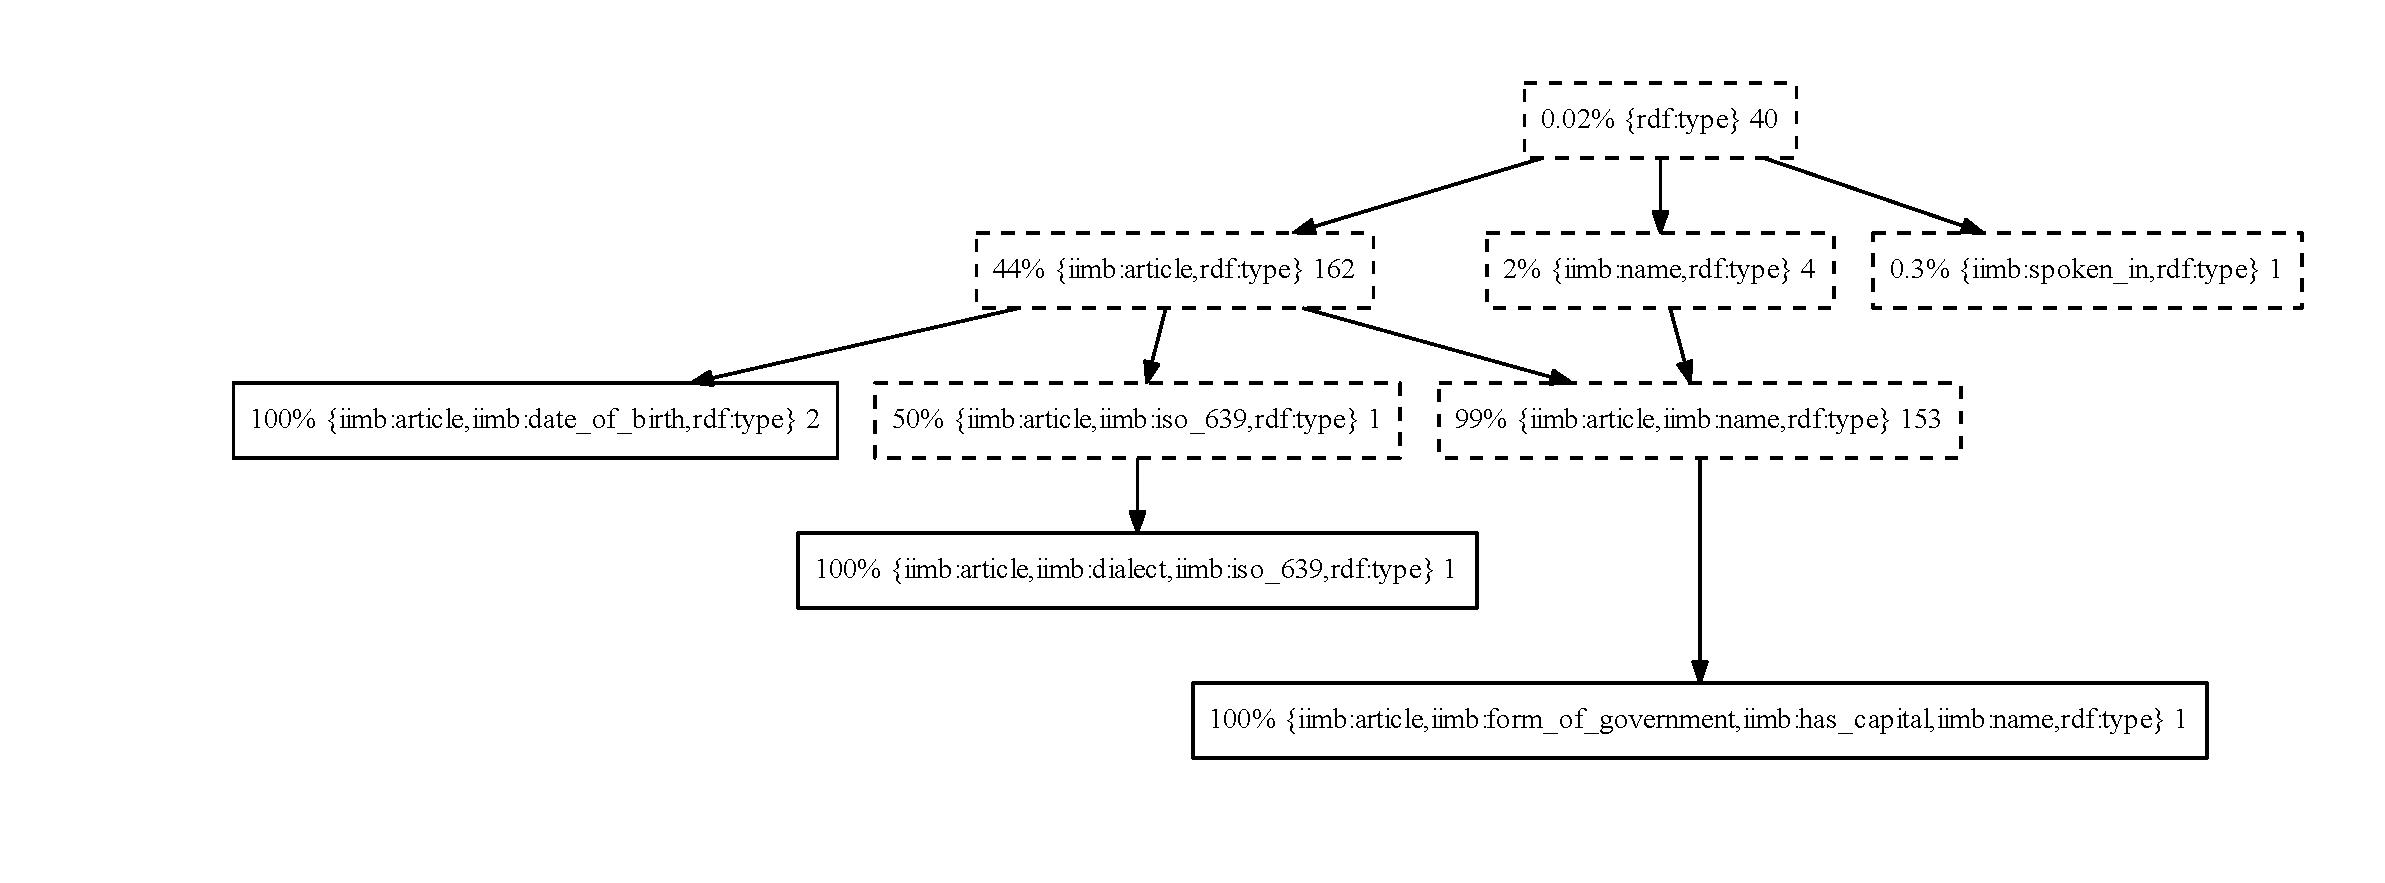
\includegraphics[width=\textwidth]{iimb_approximation_example}
\caption{An example of an indiscernibility partition for an identity relation consisting of 365 pairs. Each node is annotated with the set of predicates $P$ for which its pairs are $P$-indiscernible. The numbers of identity pairs within each partition set is displayed to the right of the predicate set label. Partition sets that contain no identity pair are not show. (This is the fourth IIMB linkset.) The number that occurs left of the predicate label in each node indicates how may pairs in that node are identity pairs. The lower approximations consists of the nodes with solid border, indicating that they contain only identity pairs. The higher approximation consists of all displayed nodes.}
\end{figure*}

\subsection{Approximation}
\label{sec:approximation}

In the previous section we partitioned a given identity relation in subrelations that can be distinguished in terms of schema predicates. In this section we create an approximation of the identity relation. This approximation will allow us to (1) give suggestions about which pairs to include in / exclude from the identity relation, and (2) give an indicator of the quality of the identity relation.

For the approximation of the identity relation we use rough set theory \cite{pawlak_1991} to represent an approximation of a given identity relation called $\approx$. The domain for our rough set approach is the Cartesian product of $S_G$. The set of predicates is the powerset of $P_G$.\footnote{Relations are called attributes in rough set theory, and they are functions that map to an arbitrary set of value labels. We only consider functions that map from binary input onto the set of Boolean truth values, and therefore use the term `predicates' to denote these functions.} This means that we have a big number of primitives to work with (quadratic in the number of constants; exponential in the number of relations).

For an arbitrary binary relation $\approx$ we can define a higher ($\overline{\approx}$, definition \ref{def:higher_approximation}) and a lower ($\underline{\approx}$, definition \ref{def:lower_approximation}) approximation of that relation. In definitions \ref{def:higher_approximation} and \ref{def:lower_approximation}, $\mathbb{R}$ characterizes a similarity relation between resource pairs. The intuition behind these definitions is that non-$\approx$-pairs that are similar to $\approx$-pairs should be in the higher approximation, whereas no $\approx$-pair that has a similar non-$\approx$-pair should be in the lower approximation.

\begin{definition}[Higher \& lower approximation]
\begin{align}
x \overline{\approx} y \  & \iff & \ 
  \exists u,v (
      \langle u, v \rangle \mathbb{R} \langle x, y \rangle
    \land
      u \approx v
  )
\label{def:higher_approximation}
\\
x \underline{\approx} y \  & \iff & \ 
  \forall u,v (
      \langle u, v \rangle \mathbb{R} \langle x, y \rangle
    \rightarrow
      u \approx v
  )
\label{def:lower_approximation}
\end{align}
\end{definition}

\begin{comment}
\begin{definition}[Higher \& lower approximation]
\label{def:higher_lower_approximation}
\begin{align}
y \in [x]_H \  \text{iff} \  \exists [u]_{\approx} (
    \vert [u]_{\approx} \vert > 1
  \land
    \mathbb{P}([u]_{\approx}) = \mathbb{P}(\{ x, y \})
  ) \\
y \in [x]_L \  \text{iff} \  \forall S \subseteq D (
    (\vert S \vert > 1 \land \mathbb{P}(S) = \mathbb{P}(\{ x, y \}))
  \rightarrow
    \exists s \in D (S = [s]_{\approx})
  )
\end{align}
\end{definition}
\end{comment}

Since we want to stay close to the traditional notion of identity, defined in terms of indiscernibility, we choose $IND(\mathcal{P}(P_G))$, defined in \ref{def:binary_indiscernibility}, as our $\mathbb{R}$.

Figure \ref{fig:iimb_example} shows an example of the lower and higher approximations for a linkset. Since in this figure a partition is only drawn when there is at least one identity pair that is indiscernible with respect to some set of predicates, the higher approximation amounts to the entire figure. The lower approximation only consists of those partition sets that contain at least one identity pair, and that contain no non-identity pair.

\subsection{Quality}
\label{sec:quality}

Given the rough set representation $\langle \underline{\approx}, \overline{\approx} \rangle$ of identity relation $\approx$, we can calculate the accuracy of this approximation with equation \ref{eq:accuracy}.

\begin{equation}
\label{eq:accuracy}
\alpha(\approx) = \frac{\vert \underline{\approx} \vert}{\vert \overline{\approx} \vert}
\end{equation}

The intuition behind the usefulness of equation \ref{eq:accuracy} is that the crispness of a set should be proportional to the quality of the identity relation on which it is based. Since a consistently applied identity relation has relatively many partition sets that contain either no identity pairs (small value for $\overline{\approx}$) or only identity pairs (big value for $\underline{\approx}$), a more consistent identity relation has a higher accuracy.

Now that we have a formal notion of identity relation quality, we can define the characteristics of an ideal identity relation. Traditionally the ideal identity relation ensures indiscernibility for all expressible properties in the language (the principle of the indiscernibility of identicals). According to this traditional view an identity relation becomes of higher quality by considering more predicates according to which two resources are not allowed to be discernible. We give a different quality criterion.

We observe that for a given equivalence relation $\approx$ defined over a domain of resources $S_G$ we can define the notion of full discernibility:

\begin{definition}[Discernible model]
\label{def:fully_discernible}
\begin{align}
& \text{A domain $S_G$ is fully discernible w.r.t.}
\nonumber
\\
& \text{a binary relation} \approx \  \text{iff}
\nonumber
\\
 & \forall x, y \in S_G (
    [x]_{\approx} = [y]_{\approx}
  \lor
    \mathbb{P}([x]_{\approx}) \neq \mathbb{P}([y]_{\approx})
  )
\end{align}
\end{definition}

For the definition it is clear that a domain of discourse is fully discernably in case there is a binary relation $\approx$ with accuracy $\alpha(\approx) = 1.0$.

\section{Experimental design}
\label{sec:experimental_design}

In section \ref{sec:research_goals} we enumerated three research goals. The first goal is met since an indiscernibility partition characterizes subrelations based on the predicates $P$ for which the pairs in that sets are $P$-indiscernible. In this way we can distinguish between different types of identity by treating $P$ as a description of a (sub)set of identity pairs.

The second goal is met since the notion of a rough set allows us to distinguish between pairs that must be in the identity relation (lower approximation) and those that may be (``not must not'', higher approximation). If we want to add/remove pairs from the identity relation, then we should not consider pairs of the former but only pairs of the latter kind.

The third goal is met since then measure for rough set accuracy is based on the discernibility criteria of an identity set. The crispness of the set is proportional to the quality of the identity relation, since a consistently applied identity relation has relatively many partition sets that contain either no identity pairs or only identity pairs.

Our approach provides a new experimental design for evaluating hypothesis that have not been evaluated before in terms of the semantics of the data.

\subsection{Hypotheses}
\label{sec:hypotheses}

Using this new approach the following hypothesis can be validated:

\begin{enumerate}
\item Take an \verb|owl:sameAs| relation and a \verb|skos:related| relation defined over the same domain. Merge them together into a new binary relation $\approx$. Establishing the lower and higher approximation of $\approx$, the hypothesis is that pairs from \verb|owl:sameAs| occur relatively more often in the lower boundary  than pairs from \verb|skos:related|.
\item Take a set of alignment pairs each of which is associated with a certain confidence measure between $0.0$ and $1.0$. Choose an arbitrary cutoff point $0.0 < c < 1.0$. The hypothesis is that alignments with a confidence larger than $c$ occur relatively more often in the lower approximation than alignments with a confidence smaller than $c$.
\item Take a set of automatically generated alignment pairs with associated confidence measures and take the gold standard or reference alignment for the same dataset. The hypothesis is that pairs that occur in the lower approximation of the alignment appear relatively more often in the gold standard that pairs that occur in the higher approximation of the alignment.
\item Another hypothesis is that the accuracy measure of a reference alignment is generally higher than the accuracy measure of an automatically generated alignment for the same dataset. A related hypothesis is that the accuracy measure is generally higher for identity relations that are considered correct by domain experts.
\end{enumerate}

\subsection{Implementation}
\label{sec:implementation}

The implementation that was built for this paper is deployed as a CPACK (extension pack) of the ClioPatria triple store \cite{schreiber_2006}. For RDF graphs that are loaded in ClioPatria this extension calculates the discernibility partition, rough set approximation and accuracy. The results are visualized using GraphViz and are displayed in a Web interface using SVG. Interactive Ajax code allows the user to click on nodes in the SVG graphic to navigate to descriptions of the resource pairs that do occur in that partition set while not being in the identity relation. This implementation should facilitate the validation of hypotheses in this new experimental setup.

\section{Conclusion}
\label{sec:conclusion}

In this paper we have given an new approach for characterizing, extending/retracting, and assessing identity relations. Our approach does this in purely qualitative terms, using schema semantics. In contemporary ontology alignment and data linking activities nonsemantic aspects of resources play a role as well. For instance similarity assessment for natural language labels is often used in data linking.

We think that the qualitative means of characterizing an identity relation are a useful addition to existing quantitative means. Also, we think that it is more useful and viable to enrich existing identity relations in the LOD based on the semantics of the graphs in which they occur, than to introduce new relationships into Semantic Web languages. Apart from the practical difficulties of teaching practitioners and transforming/enriching existing datasets, we would suggest that the meaning of an identity (sub)relation is only defined in its use, i.e., in the indiscernibility criteria it embodies.

For our approach it is not necessary to pose additional restrictions on a binary relation $\approx$. The definitions in that paper therefore apply to \verb|owl:sameAs| relations in the same way in which they would apply to \verb|skos:related| relations, or to any other binary relation.

We are currently in the process of validating the hypotheses enumerated in section \ref{sec:hypotheses}. The results of these evaluations are continuously being published on \verb|http://wouterbeek.com/identity-on-the-web/|. The website currently contains the automated results of all eighty IIMB alignments, drawn from the instance matching track of the Ontology Alignment Evaluation Initiative 2012. The website also refers to the publicly available Git repository \verb|https://github.com/wouterbeek/IOTW| where the implementation discussed in section \ref{sec:implementation} can be found.

\bibliographystyle{aaai}
\bibliography{rough_set_semantics_for_identity_management_on_the_web}

\end{document}
